\documentclass{article}
\usepackage{geometry}
%\usepackage[table]{xcolor}
\usepackage{booktabs}
\usepackage{standalone}
\usepackage{tikz}
\usepackage{subcaption}
\usepackage{siunitx}
\usetikzlibrary{patterns,snakes}

\graphicspath{{./Figures/}}

\begin{document}

\section{Ray Tracing}

\subsection{Derivation from Fermat's Principle}
Fermat's principle or the principle of least time states that the path that a ray of light takes between two points minimizes the time it takes to traverse this path. The time needed to traverse between two points is
\begin{equation}
	T = \int \! \, \mathrm{d}t = \int \! \frac{c}{c} \frac{d s / d t}{d s / d t} \, \mathrm{d}t = \frac{1}{c} \int \! \frac{c}{v} \, \mathrm{d}s = \frac{1}{c} \int \! n \, \mathrm{d}s,
	\end{equation}
where $c$ is the speed of light in a vacuum, $s$ the traversed distance, $v = d s / d t$ the speed of light in a medium and $n = c / v$ the refractive index. According to Fermat's principle the first variation of this integral must vanish,
\begin{equation}
	\delta \int \! n \, \mathrm{d} s = 0.
\end{equation}

\vspace{1cm}
To be completed 
\vspace{1cm}

\subsection{Application to the Water Tank}
Figure \ref{fig:schviepalira} shows a schematic view of a path of a light ray. The intensity of light measured at a pixel on the ccd originates from a location on the screen. We are going to construct the path of the light ray from the ccd to the screen.

\begin{figure}[hpbt]
	\includestandalone{schematicsetup}
	\caption{A schematic view of a path of a light ray (not to scale). The numbers indicate the planes through which the light ray propagates: 0, the ccd sensor inside the camera; 1, the camera lens; 2, the start of the first glass plate; 3, the end of the first glass plate; 4, the start of the second glass plate; 5, the end of the second glass plate; 6, the screen from which the light rays originate.}	
	\label{fig:schviepalira}
\end{figure}

For a given ccd sensor, we know the physical size corresponding to a pixel. When the location of the optical axis of a camera system is know, we can determine the distance to the optical axis of a pixel: $x_0$. The focal length $f$ is fixed for a given camera lens. Assuming the camera system acts as an ideal pinhole camera, the angle with which the light ray entered lens is
\begin{equation}
	\tan \phi_x = \frac{x_0}{f}.
\end{equation}
The light ray exits the camera with a position $x_1 = 0$ and an angle $\phi_x$. The index of refraction of air $n_0$ is constant. The light ray hits the first glass plate with a position
\begin{equation}
	x_2 = L_c \tan \phi_x.
\end{equation}
The index of refraction of the glass plate $n_1$ is constant. The angle under which the light ray propagates changes instantaneously, obeying Snell's law
\begin{equation}
	n_0 \sin \phi_x = n_1 \sin \phi_2.
\end{equation}

For a constant index of refraction in the water tank $n_2$ the position $x_6$ is
\begin{equation}
	x_6 (\phi_x, n_2) = (L_c+L_s) \tan \phi_x + 2 L_g \tan \arcsin \frac{n_0}{n_1} \sin \phi_x + L_t \tan \arcsin \frac{n_0}{n_2} \sin \phi_x
\end{equation}
The displacement $\Delta x$ is the difference in position $x_6$ between the constant reference state, $n_2 = n_0$, and the unknown state $n_2$, 
\begin{equation}
	\label{eq:dexcon2}
	\Delta x = x_6 (n_2 = n_0) - x_6 (n_2 = n_2) = L_t \left[ \tan \phi_x - \tan \arcsin \frac{n_0}{n_2} \sin \phi_x\right].
\end{equation}

For a varying index of refraction in the water tank $n_2 = n_2(\underline{x})$, the position $x_6$ is

\vspace{1cm}
To be completed 
\vspace{1cm}

\subsection{Displacements expected from Theory}
Substituting some characteristic values into (\ref{eq:dexcon2}) we obtain the displacements expected from theory. Figure \ref{fig:1} shows the expected displacements for fresh water $n_2 = 1.333$ compared to a reference state of air $n_2 = 1.0$. The water acts as a magnification glass: all the displacements are away from the optical axis, located in the middle of each figure. 

Figure \ref{fig:2} shows the expected displacements for water with a maximum of salt added $n_2 = 1.4$. The displacement pattern looks the same as the fresh water pattern. The magnitude of displacement is slightly larger. 

Comparing \ref{fig:1} and \ref{fig:2}, which show the minimum and maximum index of refraction obtainable for water with salts, the displacements have the same pattern and their maximum magnitudes are similar: around \SI{7}{\milli\metre} for $n_2 = 1.333$ and around \SI{8}{\milli\metre} for $n_2 = 1.4$.

Figure \ref{fig:3} shows the expected displacement for salt water with $n_2 = 1.4$ compared to a reference state of fresh water $n_2 = 1.333$. 

\begin{figure}
\begin{subfigure}[b]{.5\linewidth}
\centering 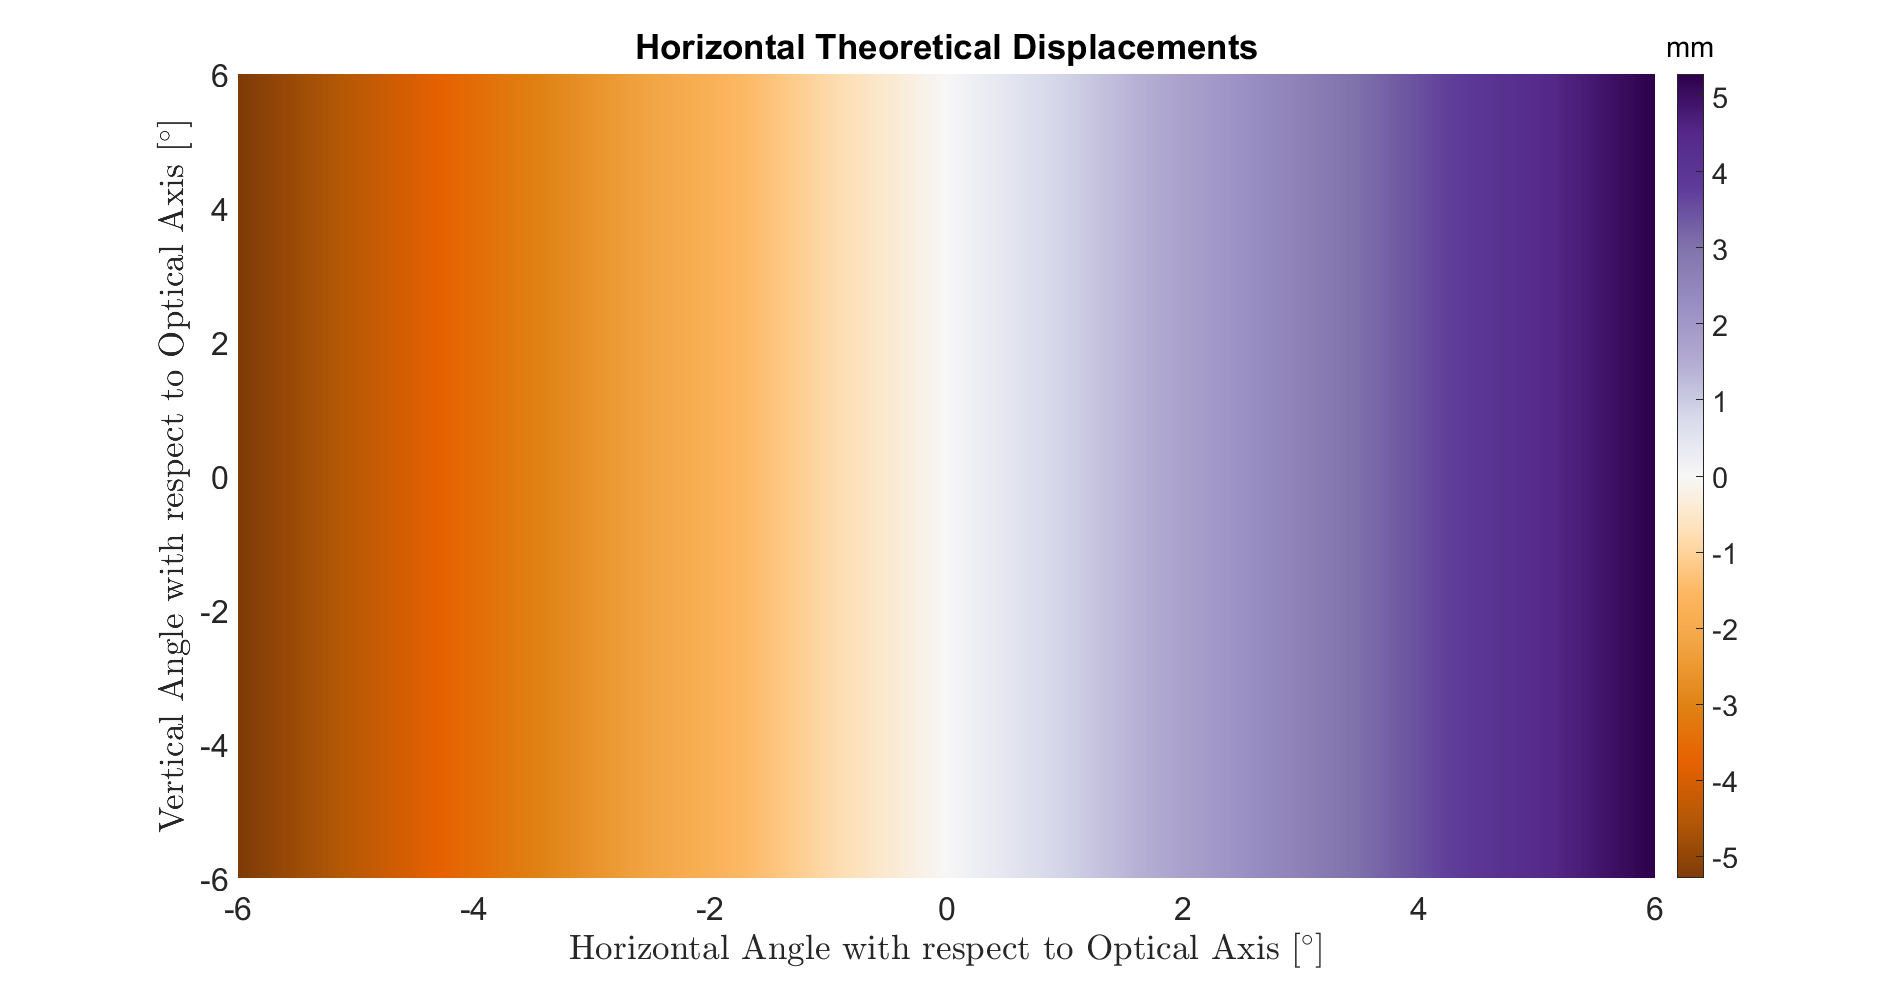
\includegraphics[width=\linewidth]{hordispnmin.png}
\caption{Horizontal Displacements.}\label{fig:1a}
\end{subfigure}%
\begin{subfigure}[b]{.5\linewidth}
\centering\large 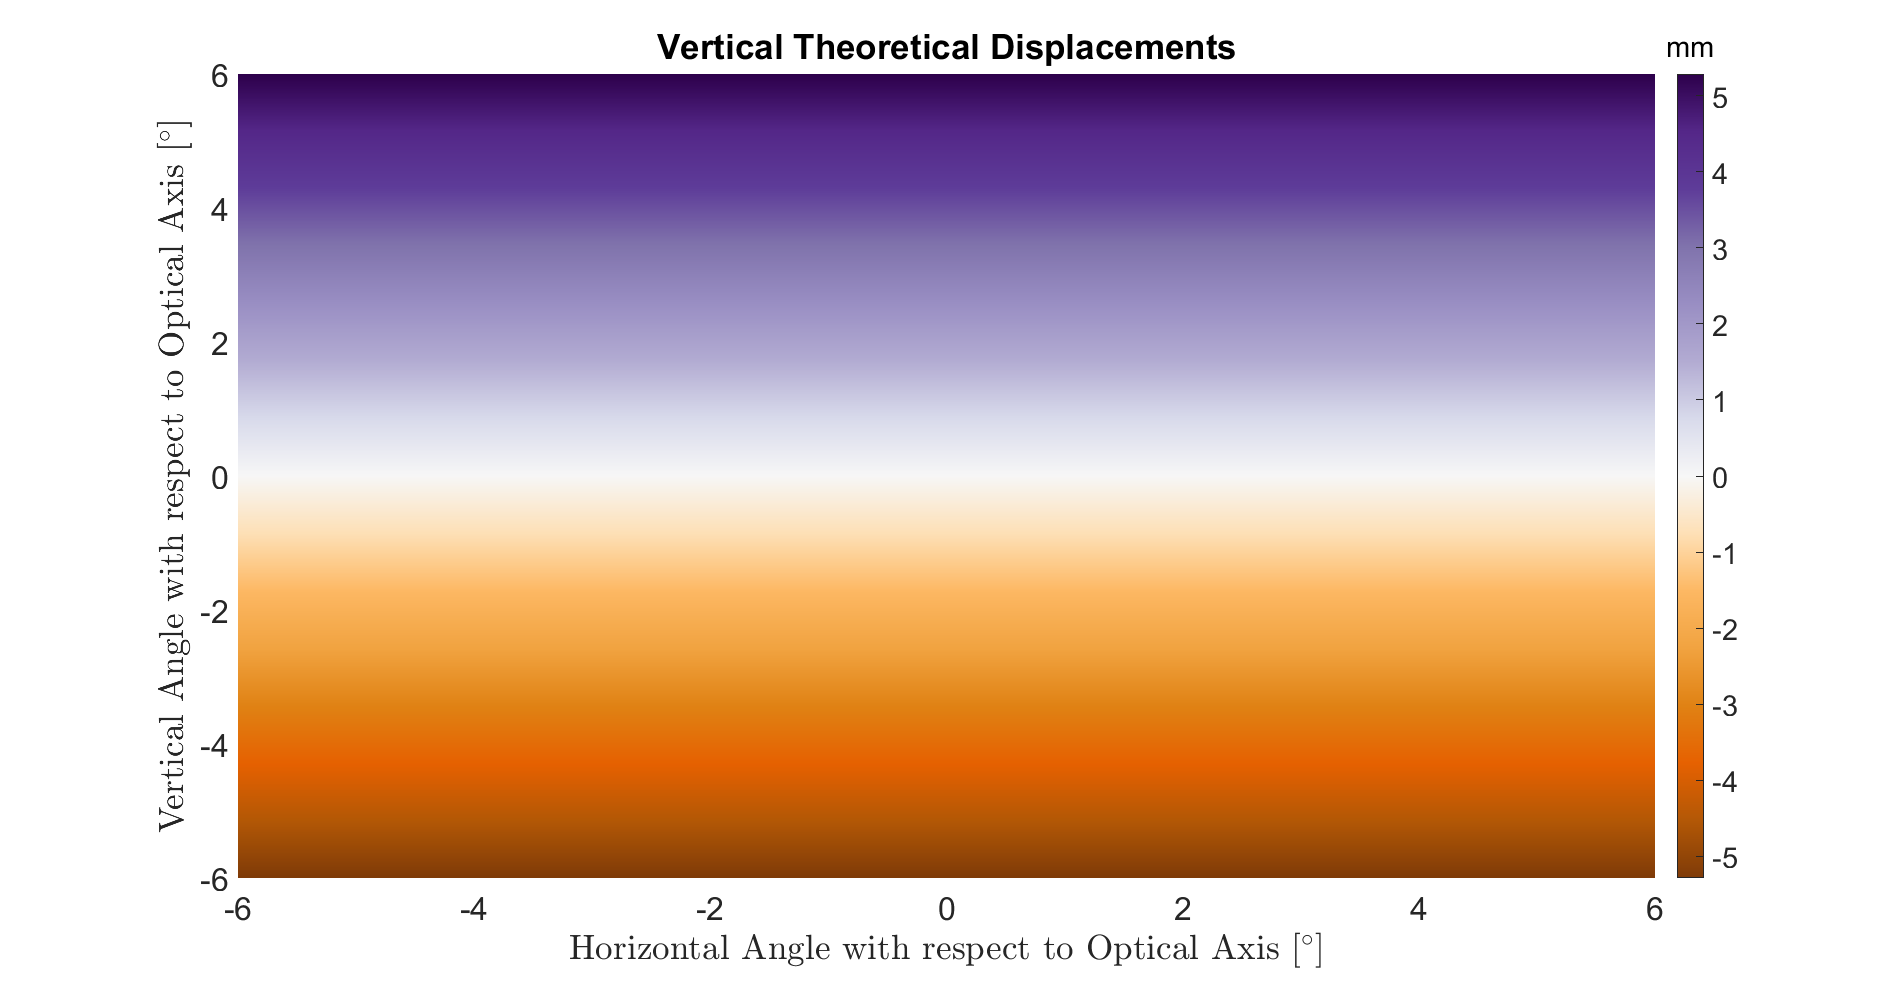
\includegraphics[width=\linewidth]{verdispnmin.png}
\caption{Vertical Displacements.}\label{fig:1b}
\end{subfigure} \\
\begin{subfigure}[b]{\linewidth}
\centering 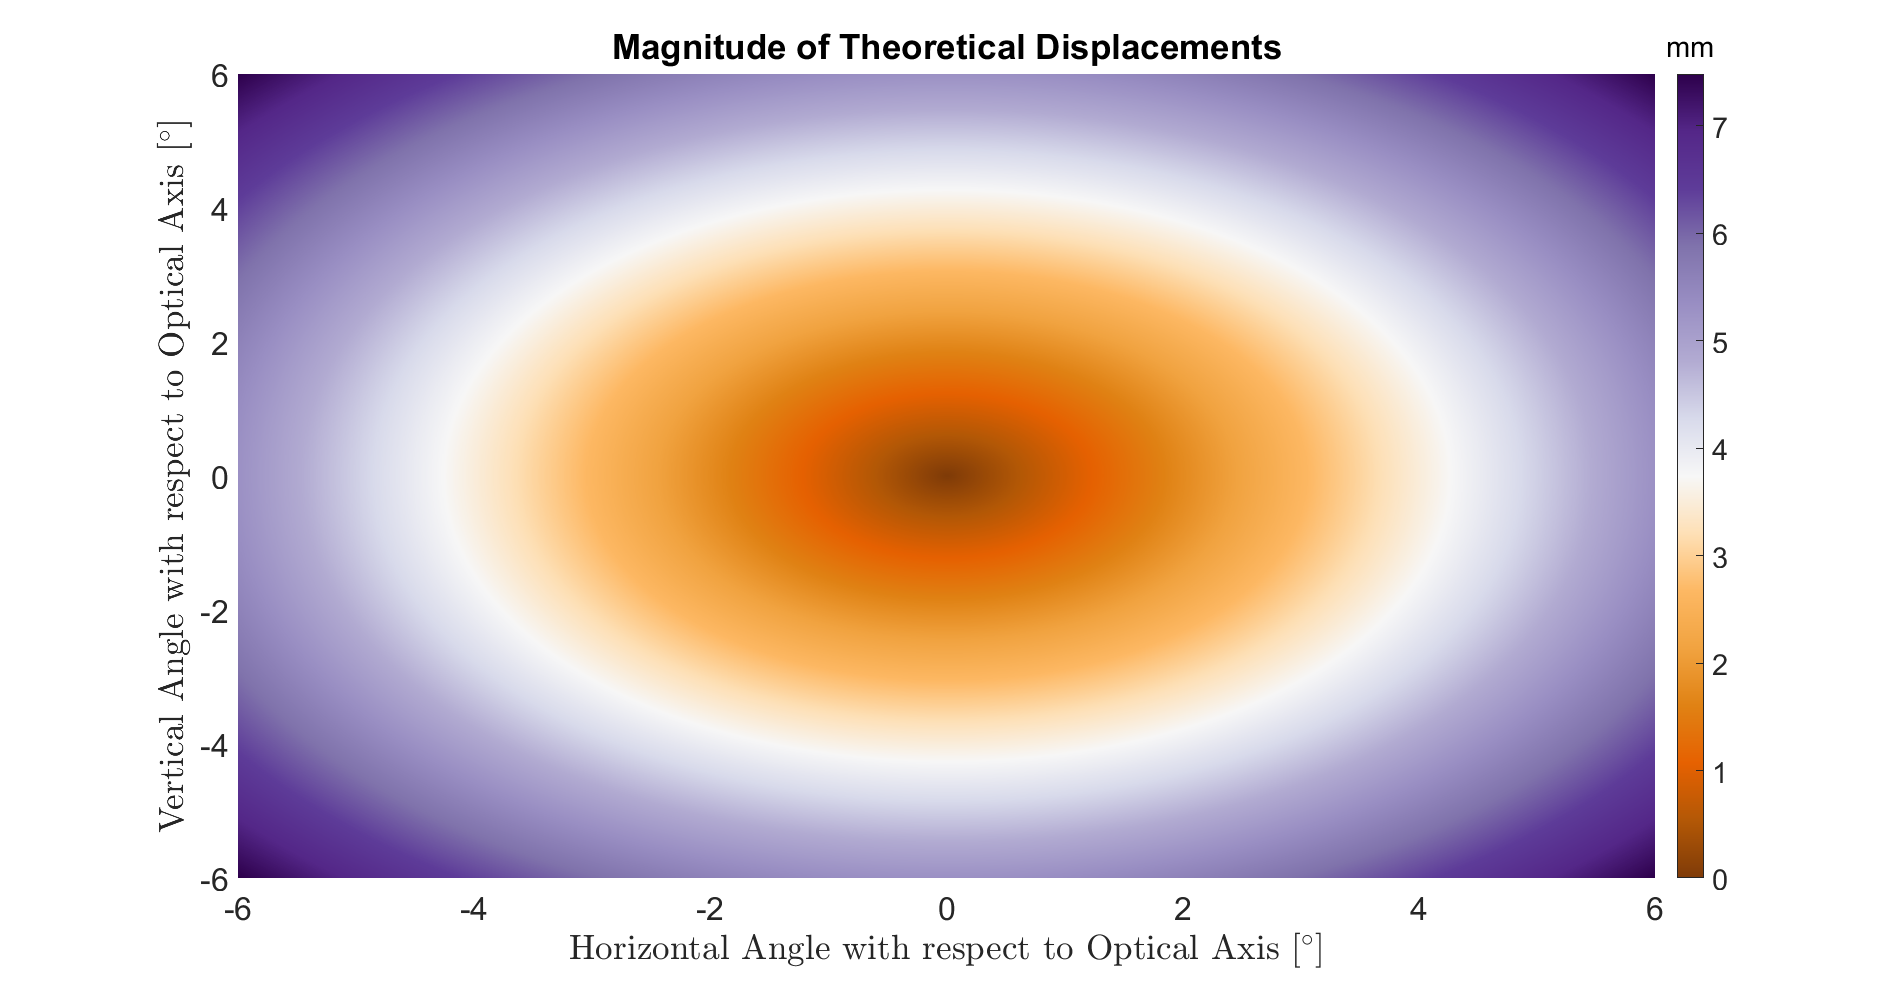
\includegraphics[width=\linewidth]{magndispnmin.png}
\caption{Magnitude of Displacements.}\label{fig:1c}
\end{subfigure}%
\caption{Displacements expected from theory for $n_2 = 1.333$ and $L_t = \SI{0.2}{m}$.}\label{fig:1}
\end{figure}

\begin{figure}
\begin{subfigure}[b]{.5\linewidth}
\centering 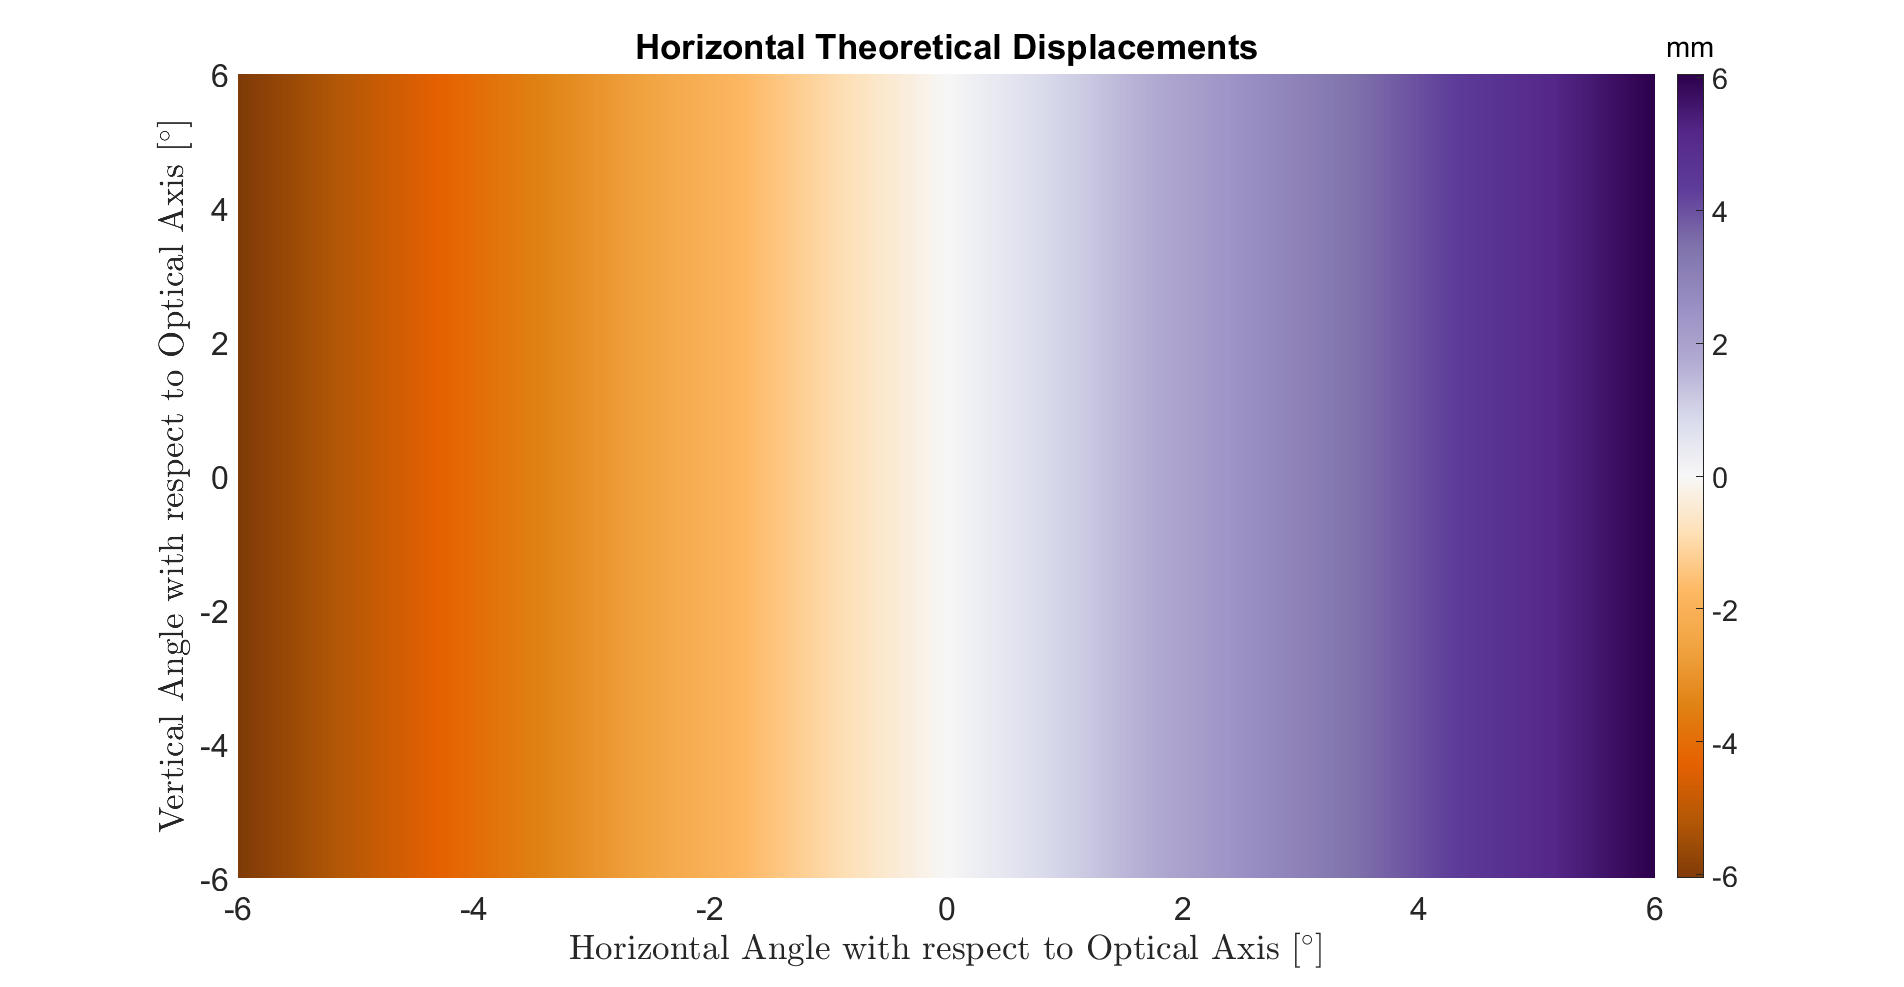
\includegraphics[width=\linewidth]{hordispnmax.png}
\caption{Horizontal Displacements.}\label{fig:2a}
\end{subfigure}%
\begin{subfigure}[b]{.5\linewidth}
\centering\large 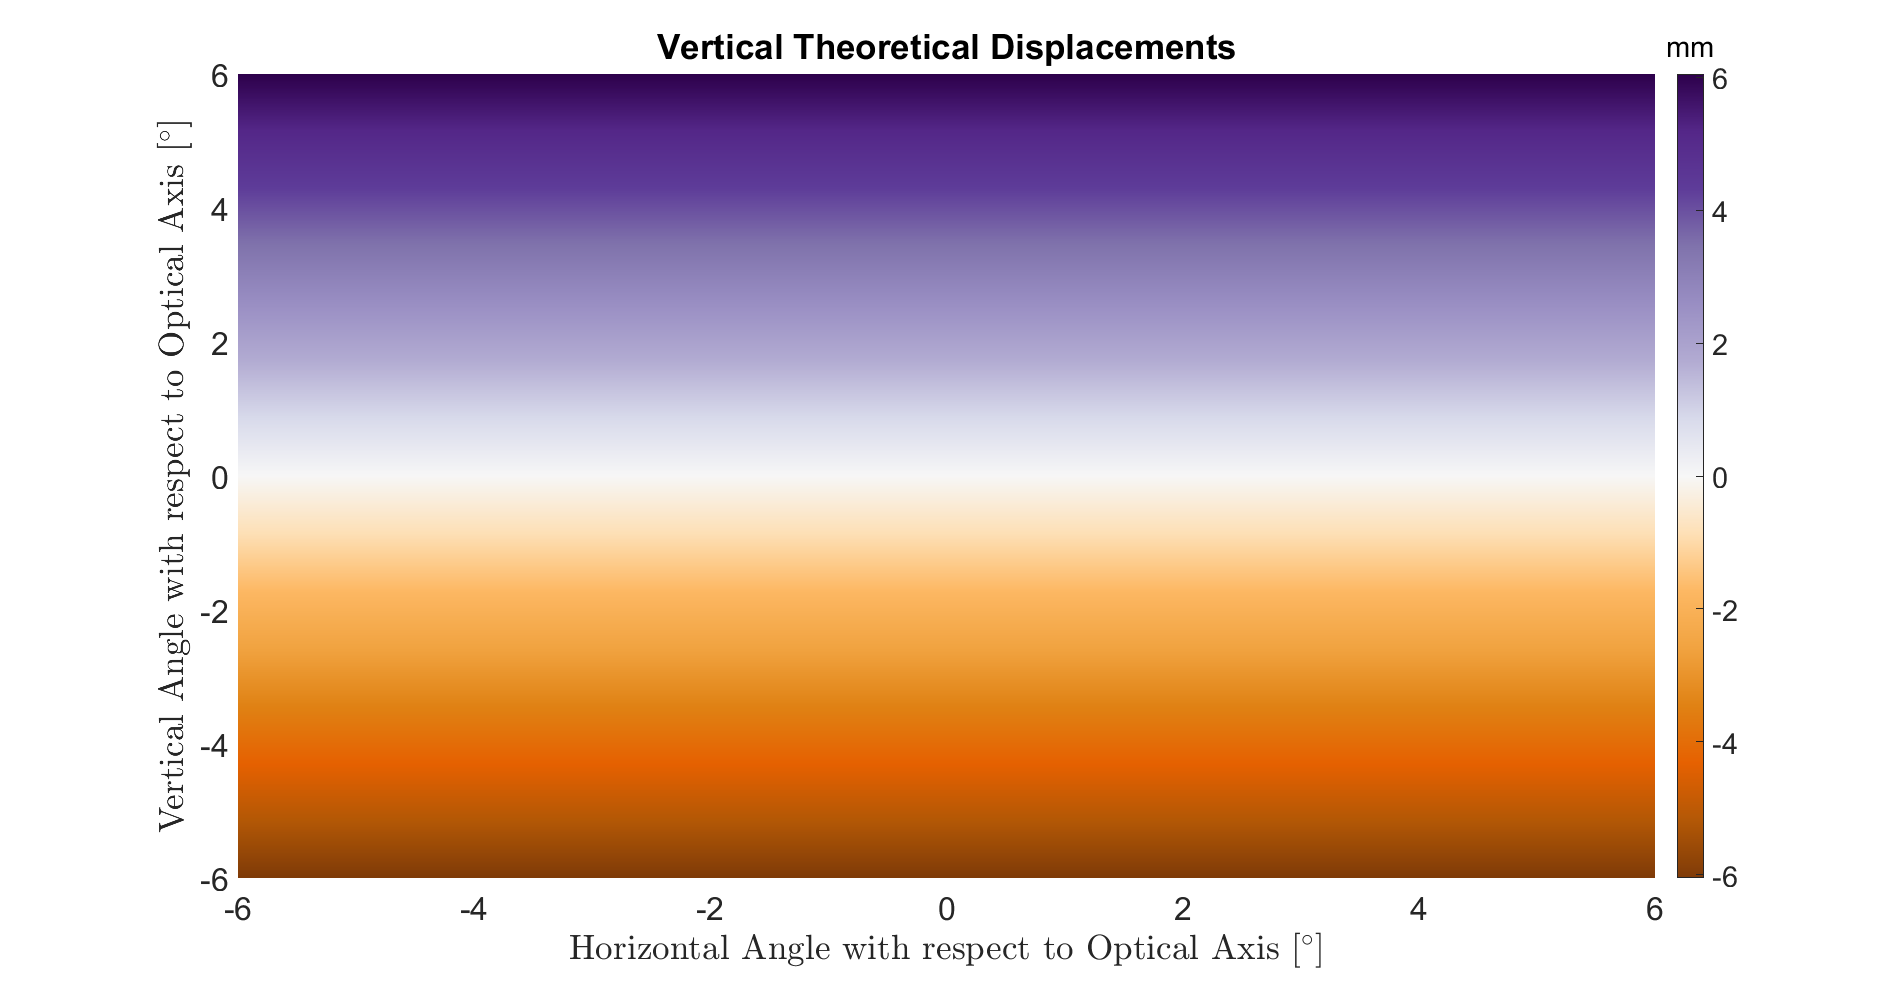
\includegraphics[width=\linewidth]{verdispnmax.png}
\caption{Vertical Displacements.}\label{fig:2b}
\end{subfigure} \\
\begin{subfigure}[b]{\linewidth}
\centering 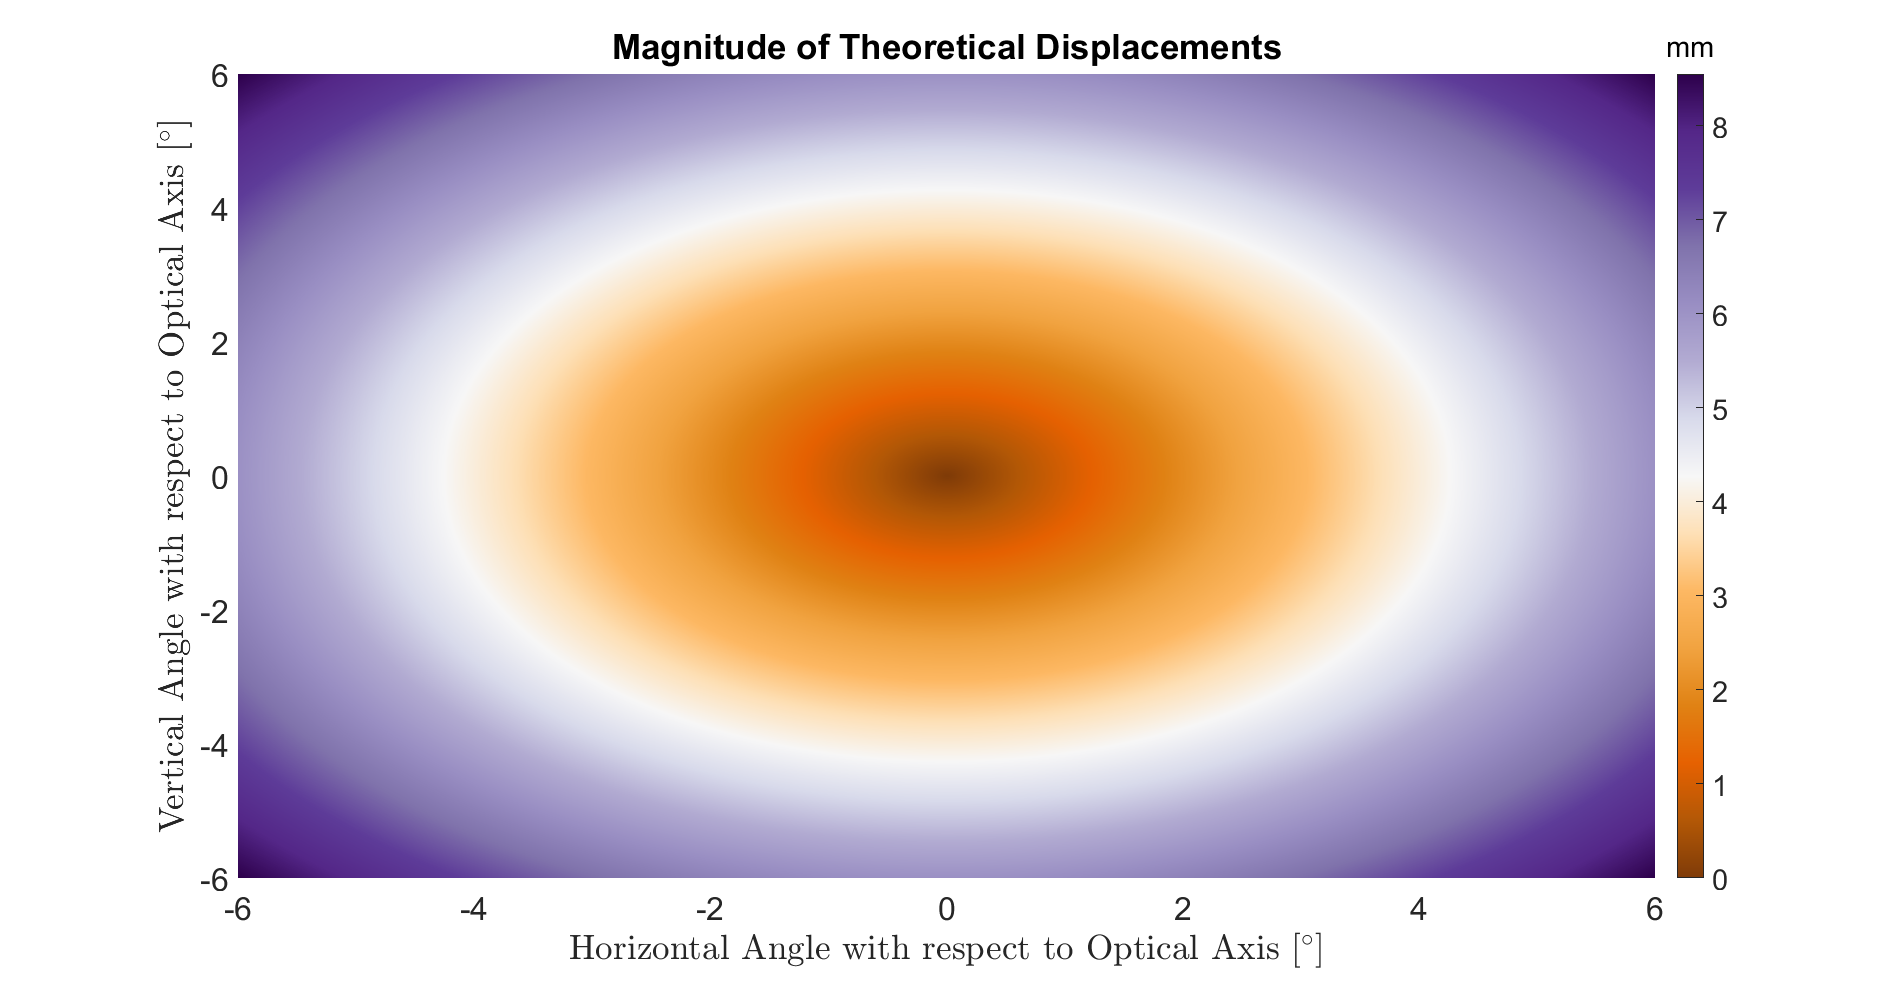
\includegraphics[width=\linewidth]{magndispnmax.png}
\caption{Magnitude of Displacements.}\label{fig:2c}
\end{subfigure}%
\caption{Displacements expected from theory for $n_2 = 1.4$ and $L_t = \SI{0.2}{m}$.}\label{fig:2}
\end{figure}

\begin{figure}
\begin{subfigure}[b]{.5\linewidth}
\centering 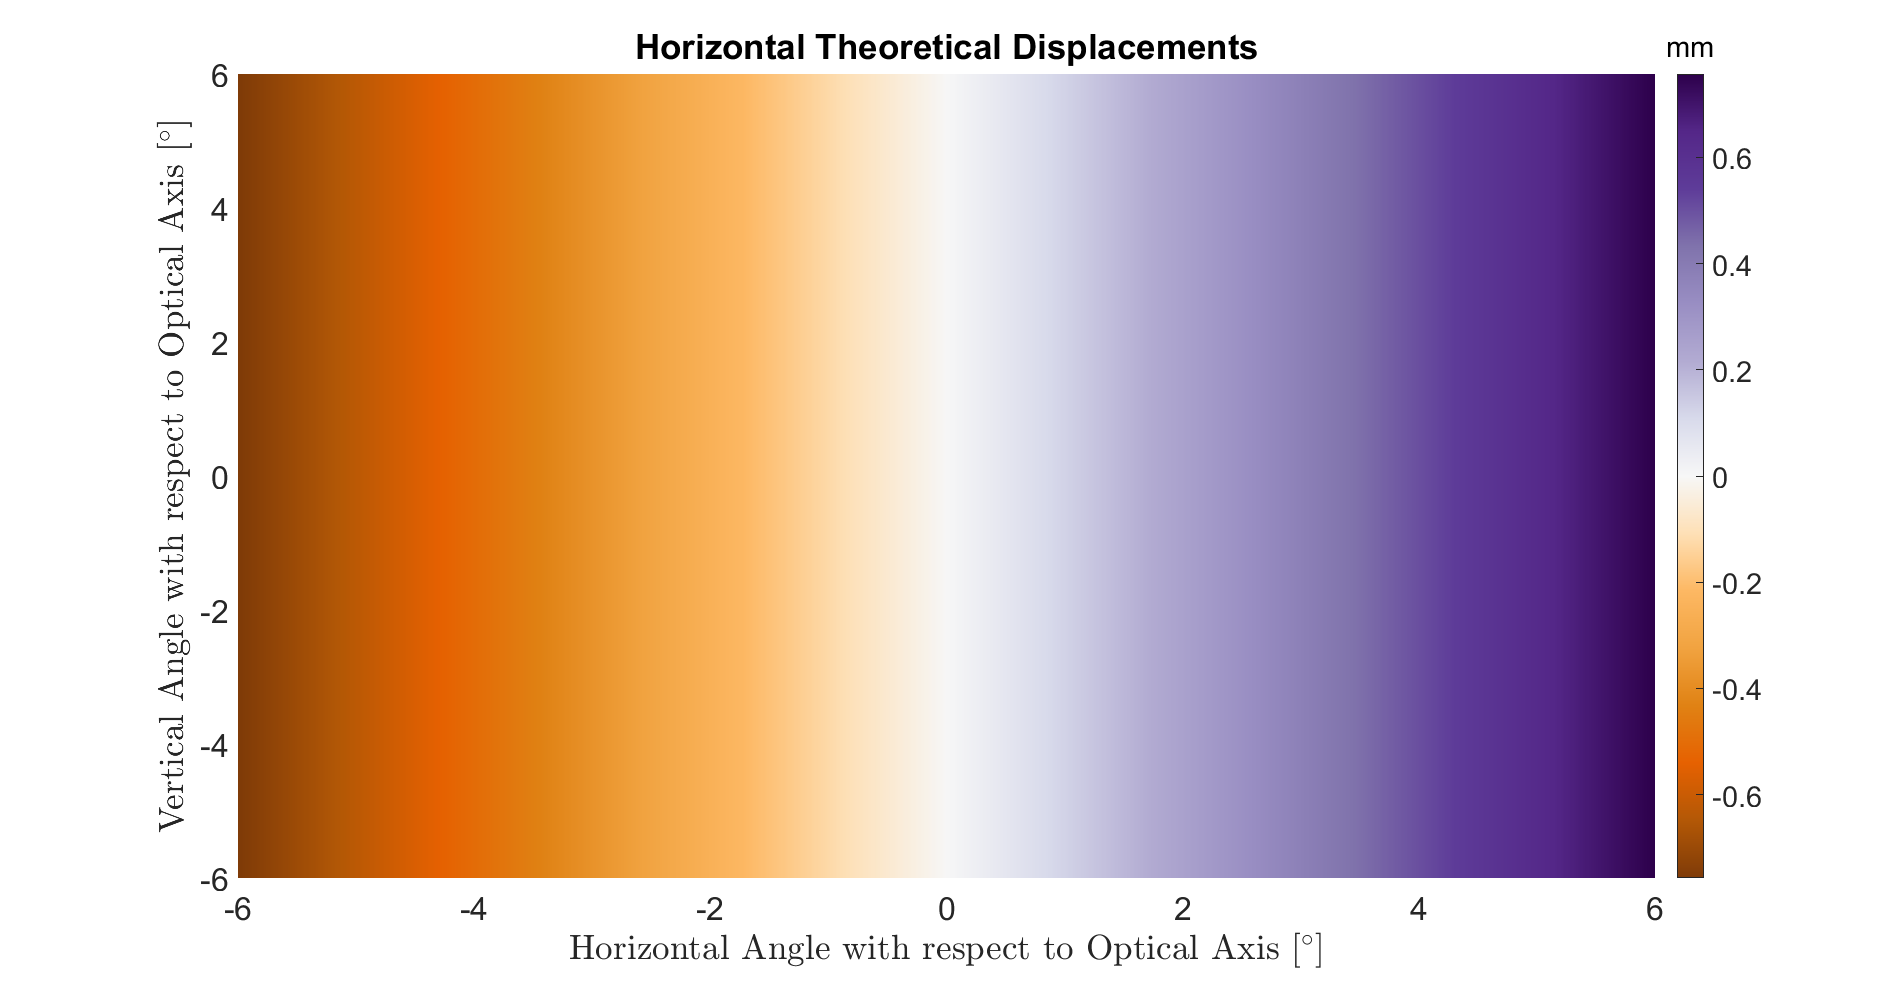
\includegraphics[width=\linewidth]{hordispnmaxrefstatenmin.png}
\caption{Horizontal Displacements.}\label{fig:3a}
\end{subfigure}%
\begin{subfigure}[b]{.5\linewidth}
\centering\large 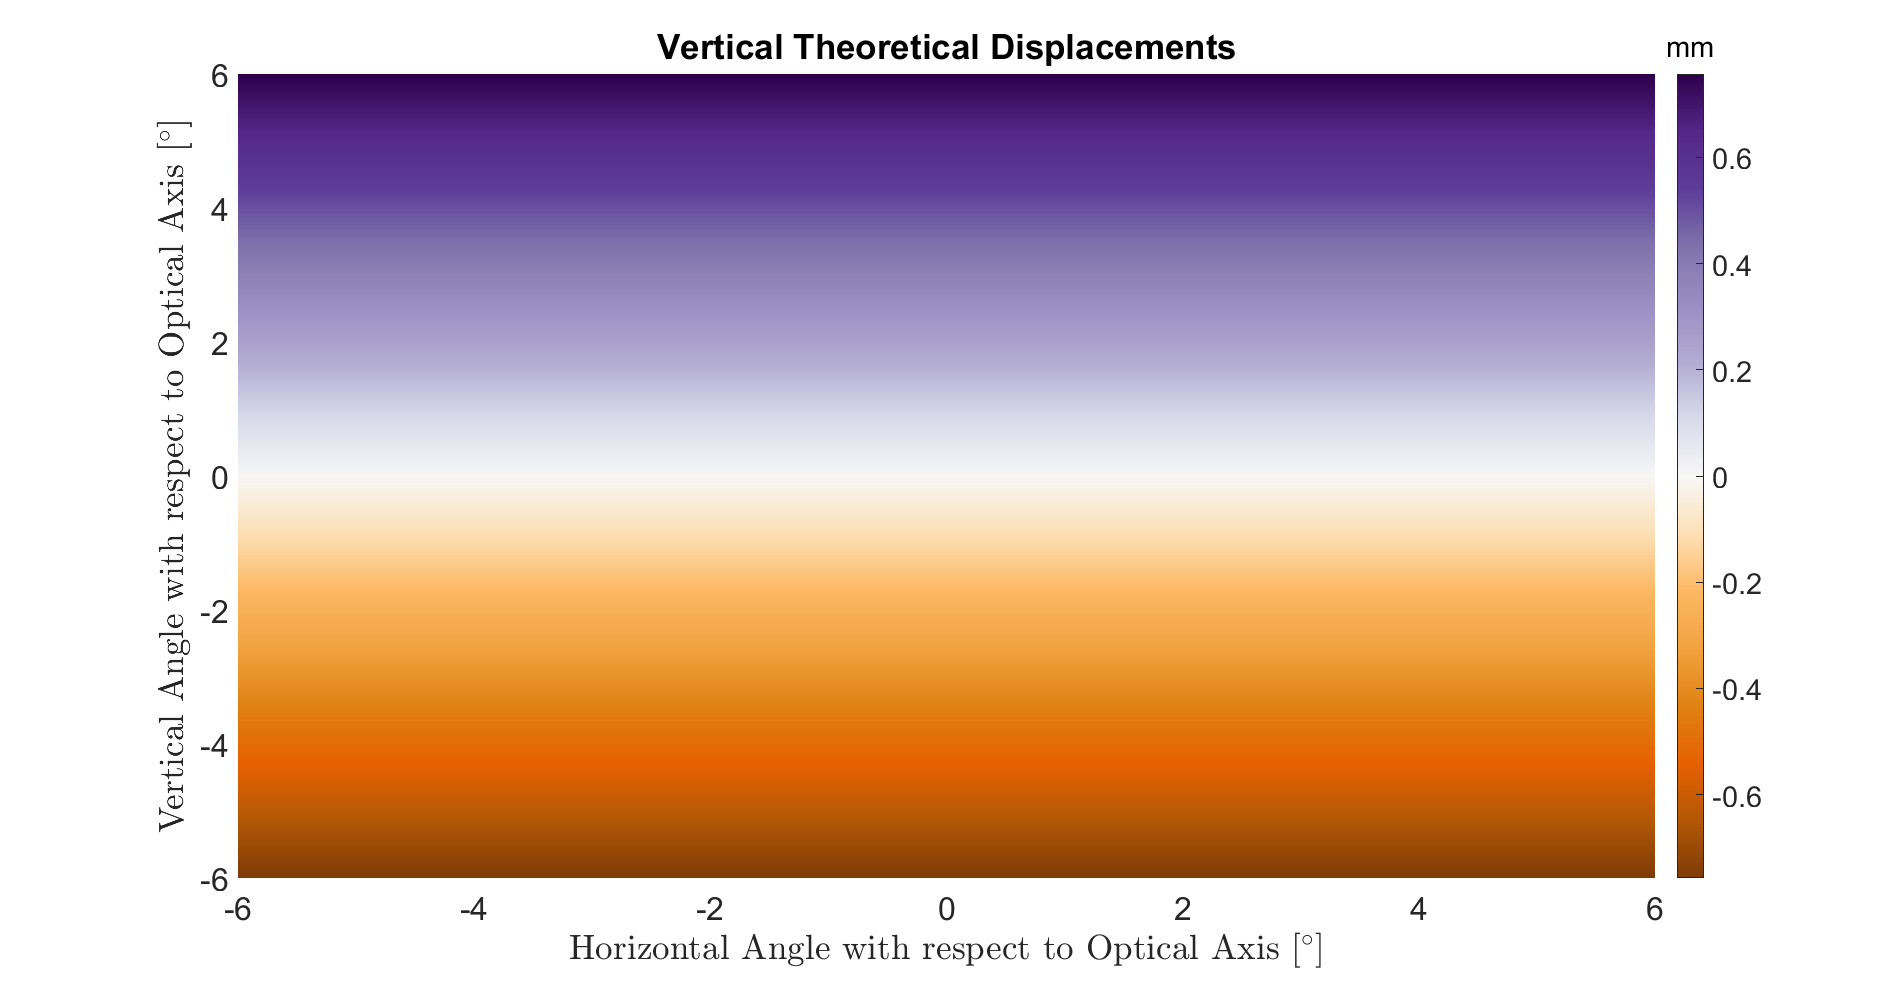
\includegraphics[width=\linewidth]{verdispnmaxrefstatenmin.png}
\caption{Vertical Displacements.}\label{fig:3b}
\end{subfigure} \\
\begin{subfigure}[b]{\linewidth}
\centering 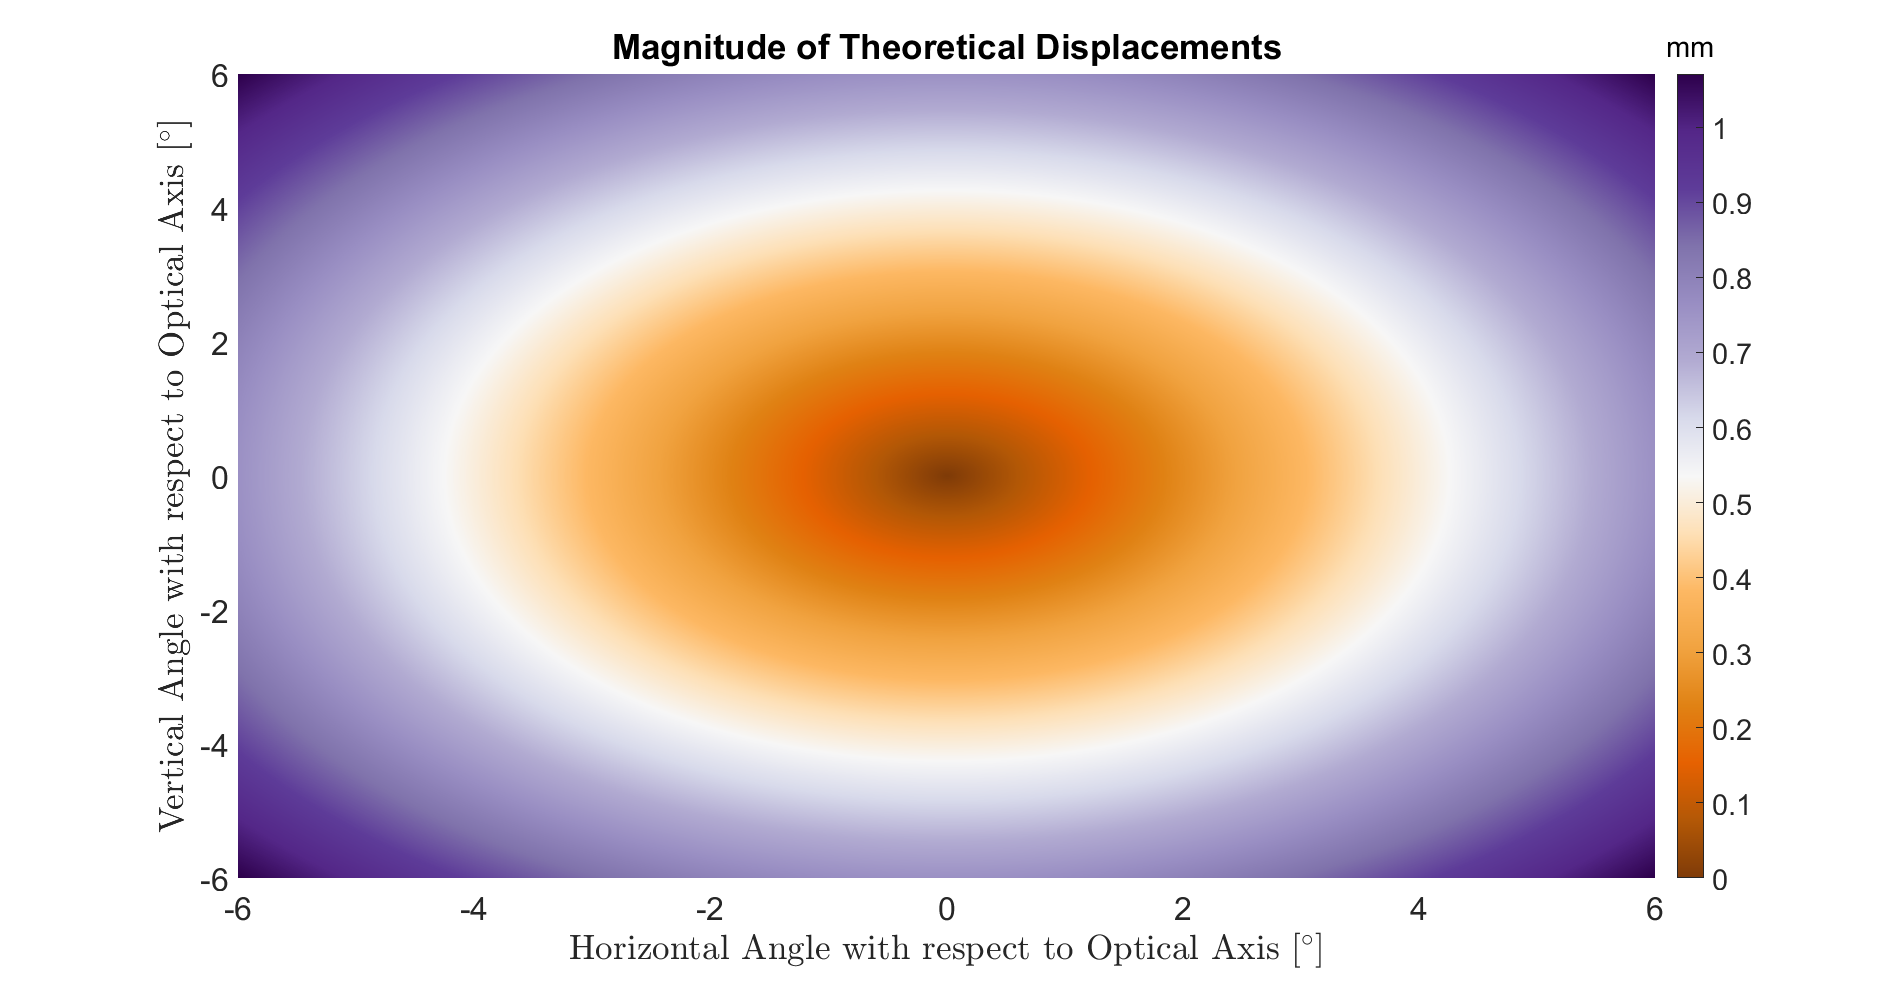
\includegraphics[width=\linewidth]{magndispnmaxrefstatenmin.png}
\caption{Magnitude of Displacements.}\label{fig:3c}
\end{subfigure}%
\caption{Displacements expected from theory using fresh water as the reference state for $n_2 = 1.4$ and $L_t = \SI{0.2}{m}$.}\label{fig:3}
\end{figure}

Looking at (\ref{eq:dexcon2}), we see that there are two main uncertainties when determining the index of refraction $n_2$: (1) uncertainty in the displacements $\Delta x$ and (2) uncertainty in the angles $\phi_x$. To get a feeling for these uncertainties, we chose an $n_2$, computed a displacement field using (\ref{eq:dexcon2}), added an uncertainty and computed $n_2$ by inverting (\ref{eq:dexcon2}). 

First, we added white noise to the displacement field. Figure \ref{fig:nfromhordispnoise} shows the index of refraction obtained from the horizontal displacements when adding this noise. Around the center line, where both the displacements $\Delta x$ and the angles $\phi_x$ are near zero, the errors are largest. This error band around the center line also exists for the index of refraction obtained from the vertical displacements. There, the error band is horizontal. When combining the horizontal and vertical displacements into a magnitude of displacements the horizontal and vertical error bands disappear, except for where they overlap: near the centerpoint we are left with a region of large errors due noise: both the displacements and the angles are near zero. 

Second, we added a shift in the optical axis. Figure \ref{fig:nfrommagndispnoiseshift} shows the index of refraction obtained from a small shift (both horizontal and vertical) in the optical axis. A very recognizable pattern appears: a figure eight. The orientation of the eight is determined by the shift in the optical axis. 


\begin{figure}
\centering 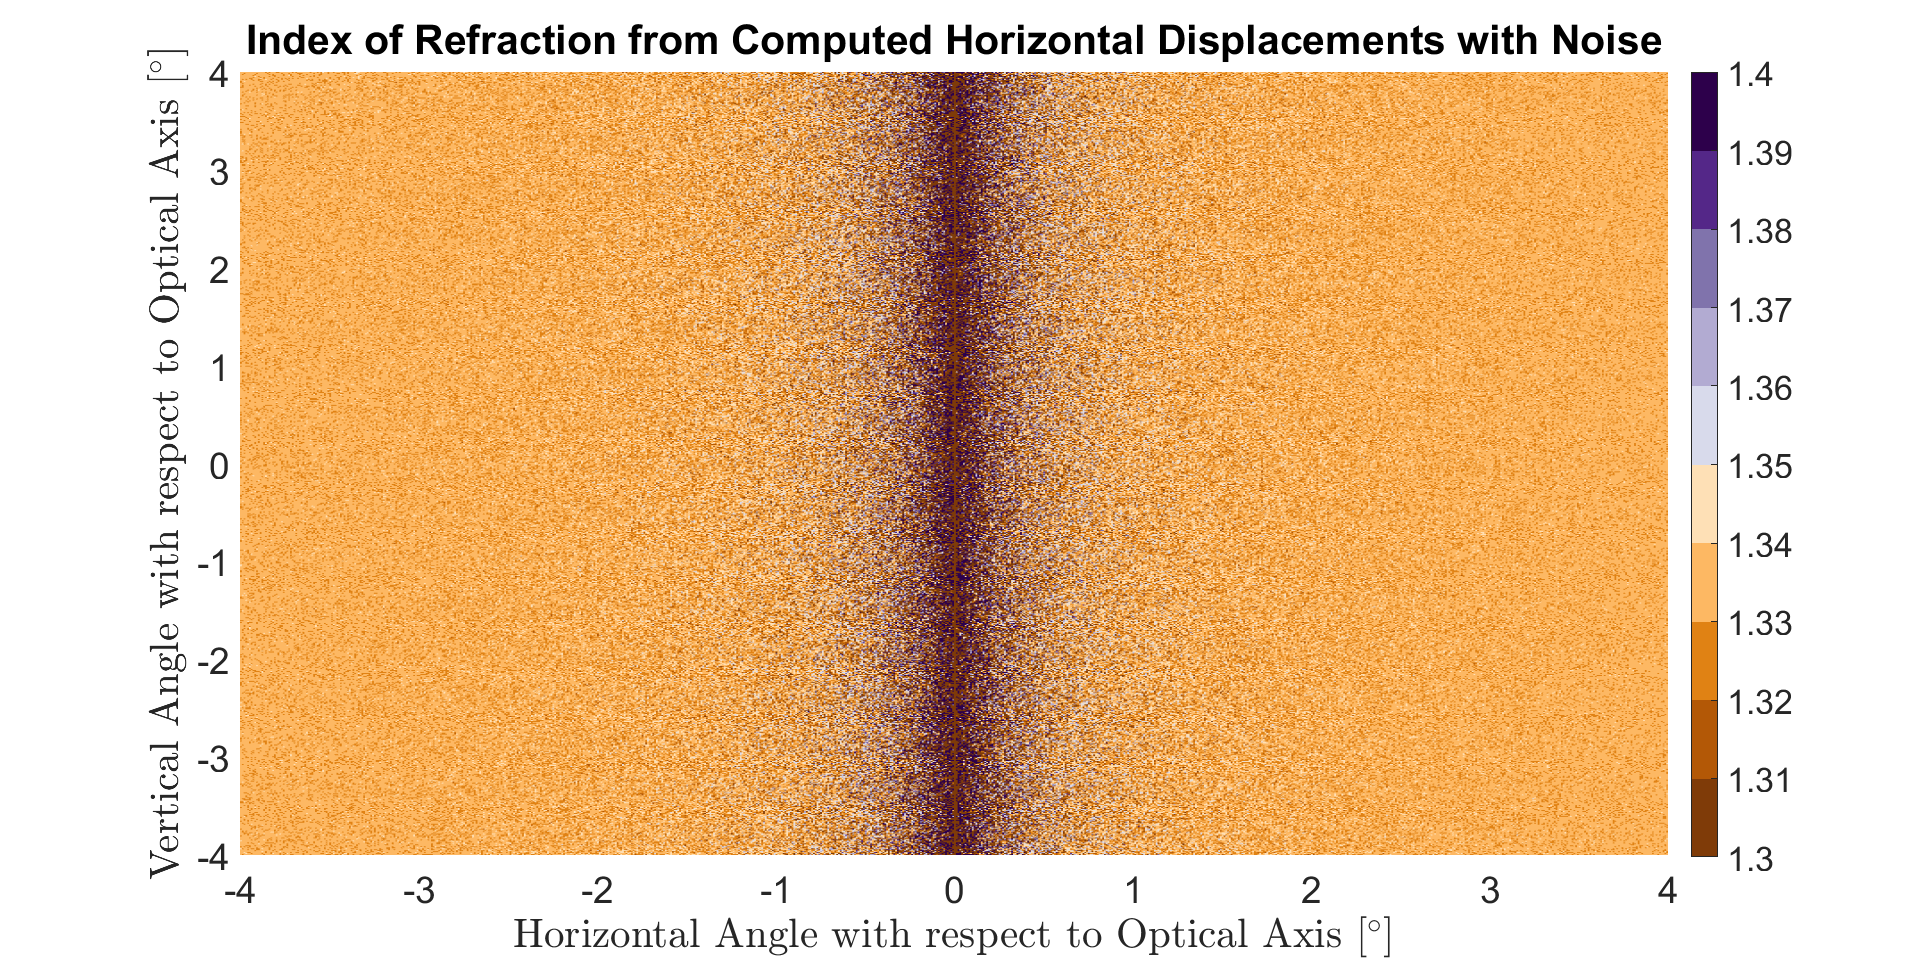
\includegraphics[width=\linewidth]{nfromhordispnoise.png}
\caption{Index of Refraction determined from Computed Horizontal Displacements with Noise.}
\label{fig:nfromhordispnoise}
\end{figure}

\begin{figure}
\centering 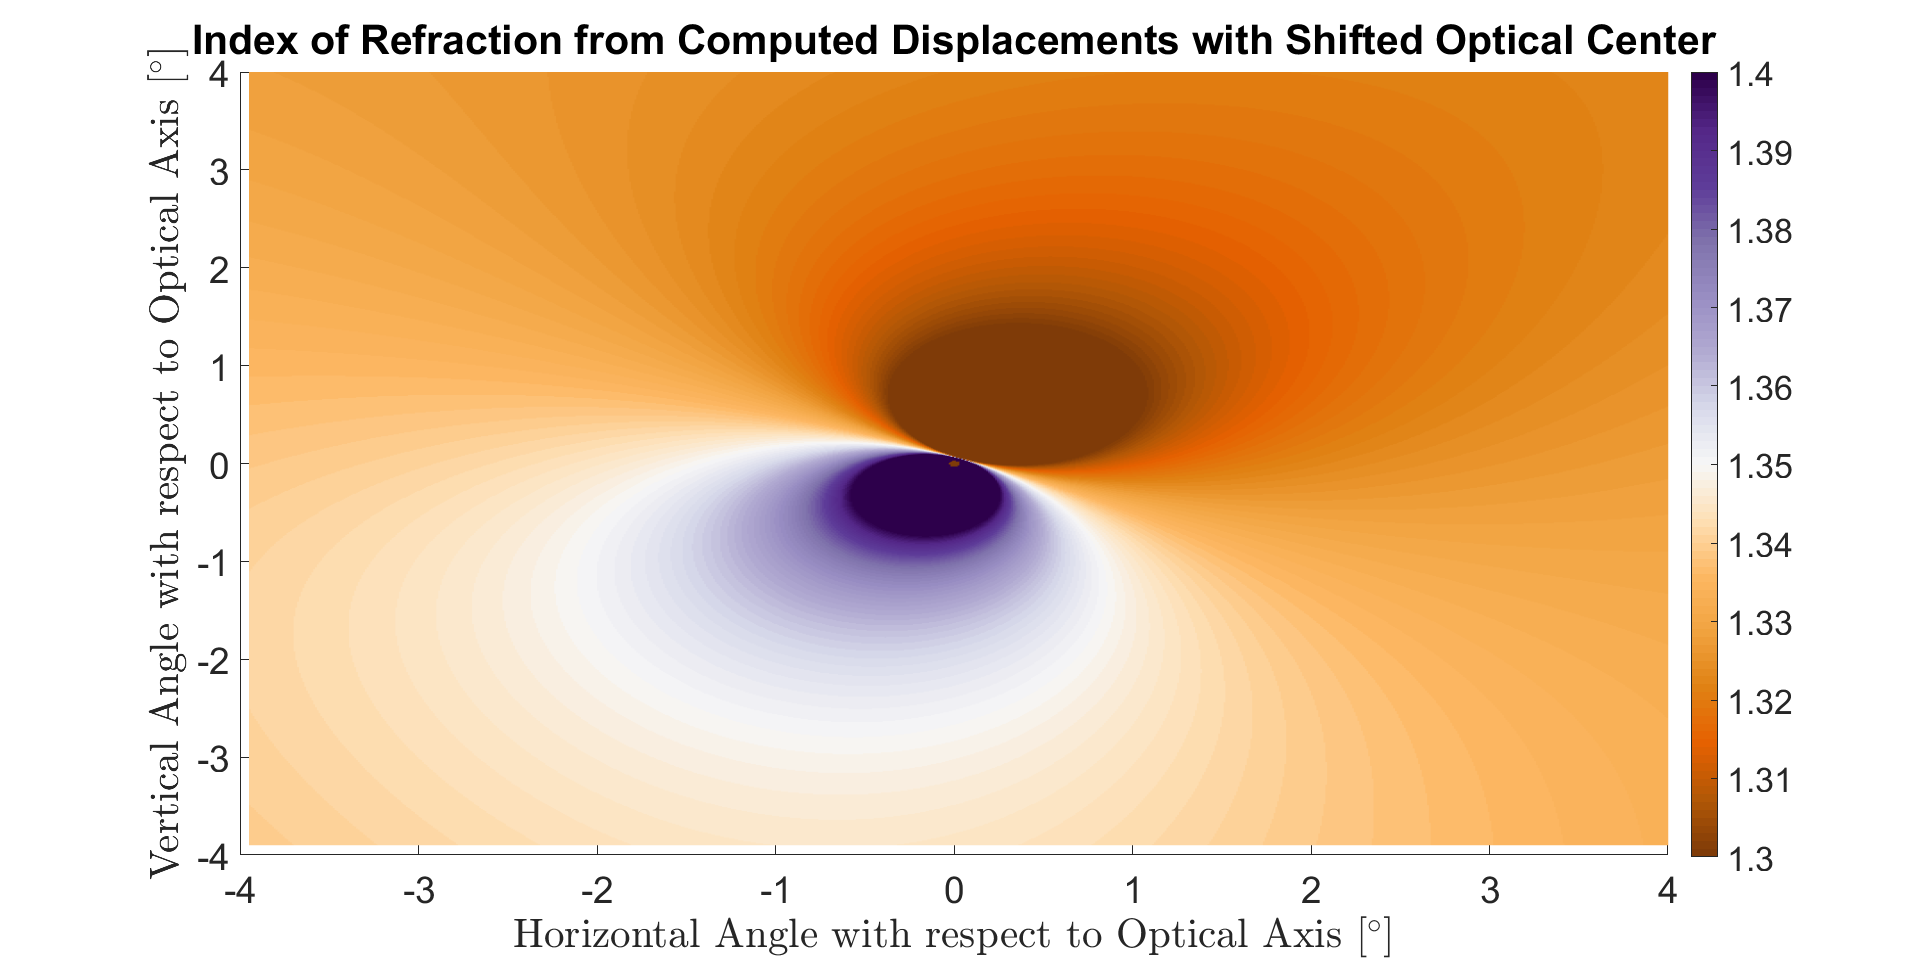
\includegraphics[width=\linewidth]{nfrommagndispshift.png}
\caption{Index of Refraction determined from Computed Displacements with a Shift in the Optical Center.}
\label{fig:nfrommagndispnoiseshift}
\end{figure}

Last, we combine white noise with a shift in optical axis, shown in Figure \ref{fig:nfrommagndispnoiseshift} with data obtained in the lab, shown in Figure \ref{fig:nfrommdataexample}. In the lab data, we see the figure eight appearing, indicating an error in the determination of the optical axis.  

\begin{figure}
\centering 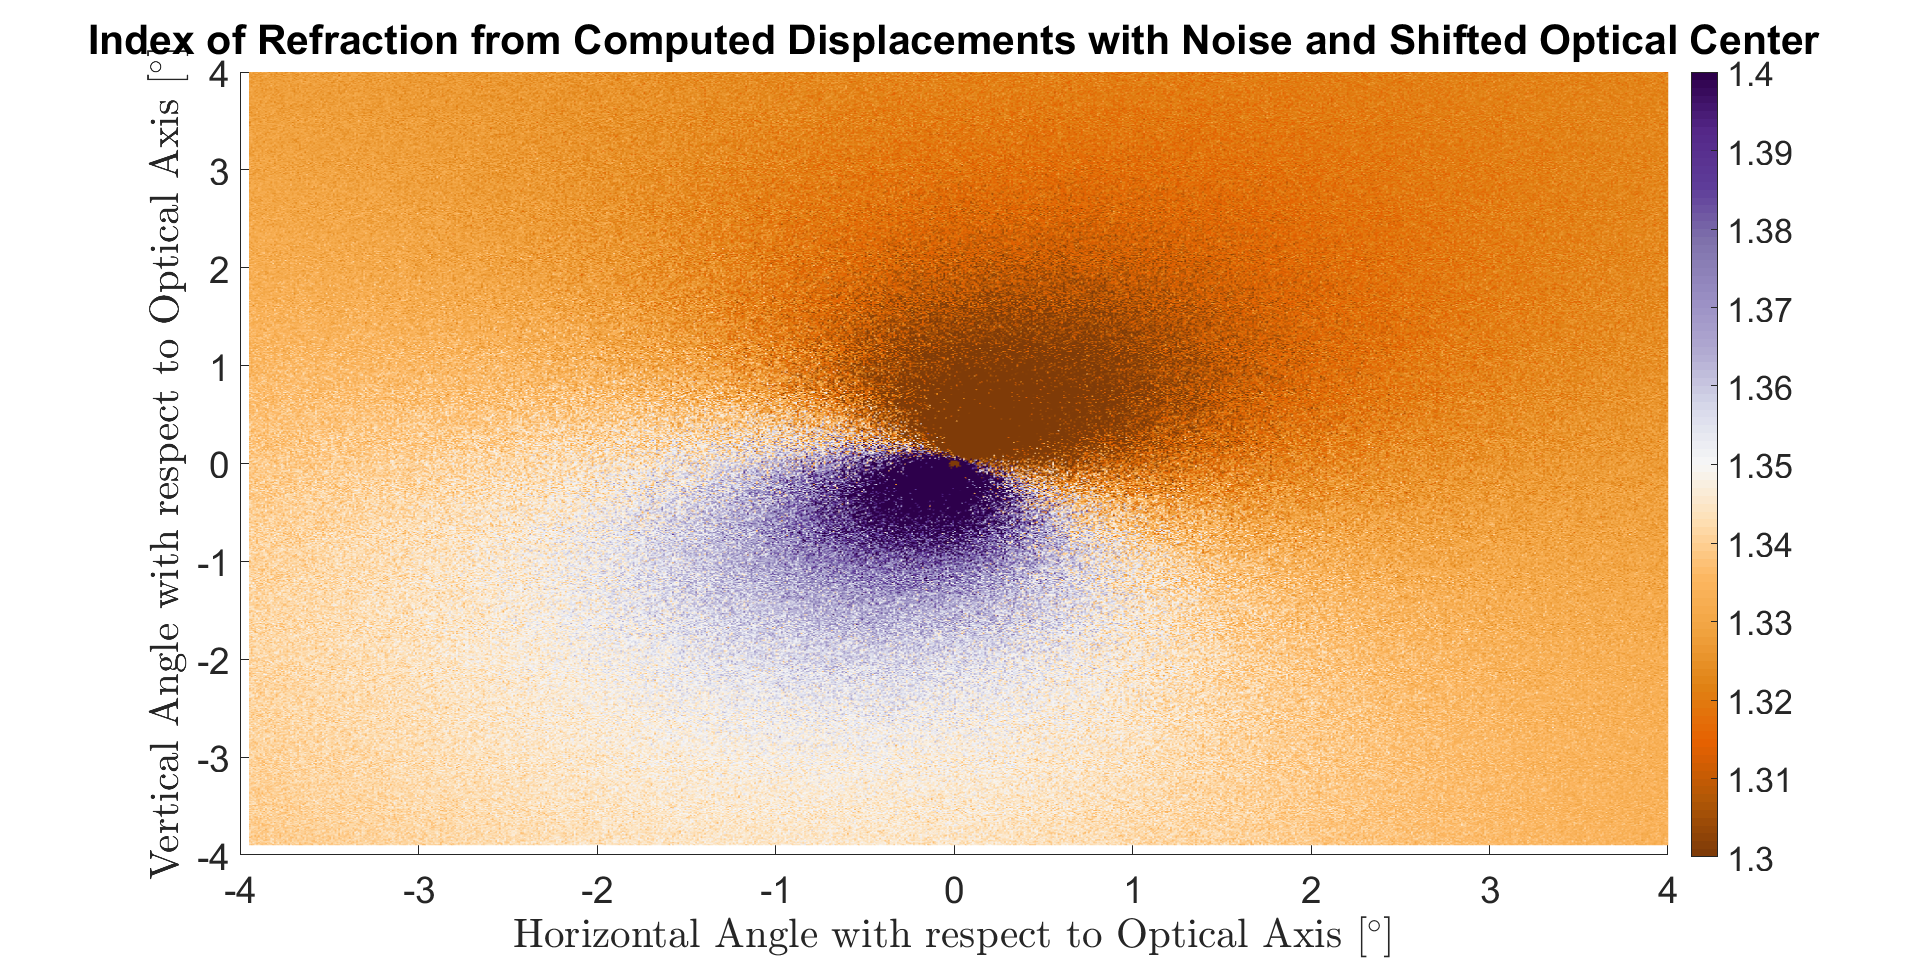
\includegraphics[width=\linewidth]{nfrommagndispnoiseshift.png}
\caption{Index of Refraction determined from Computed Displacements with Noise and a Shift in the Optical Center.}
\label{fig:nfrommagndispnoiseshift}
\end{figure}

\begin{figure}
\centering 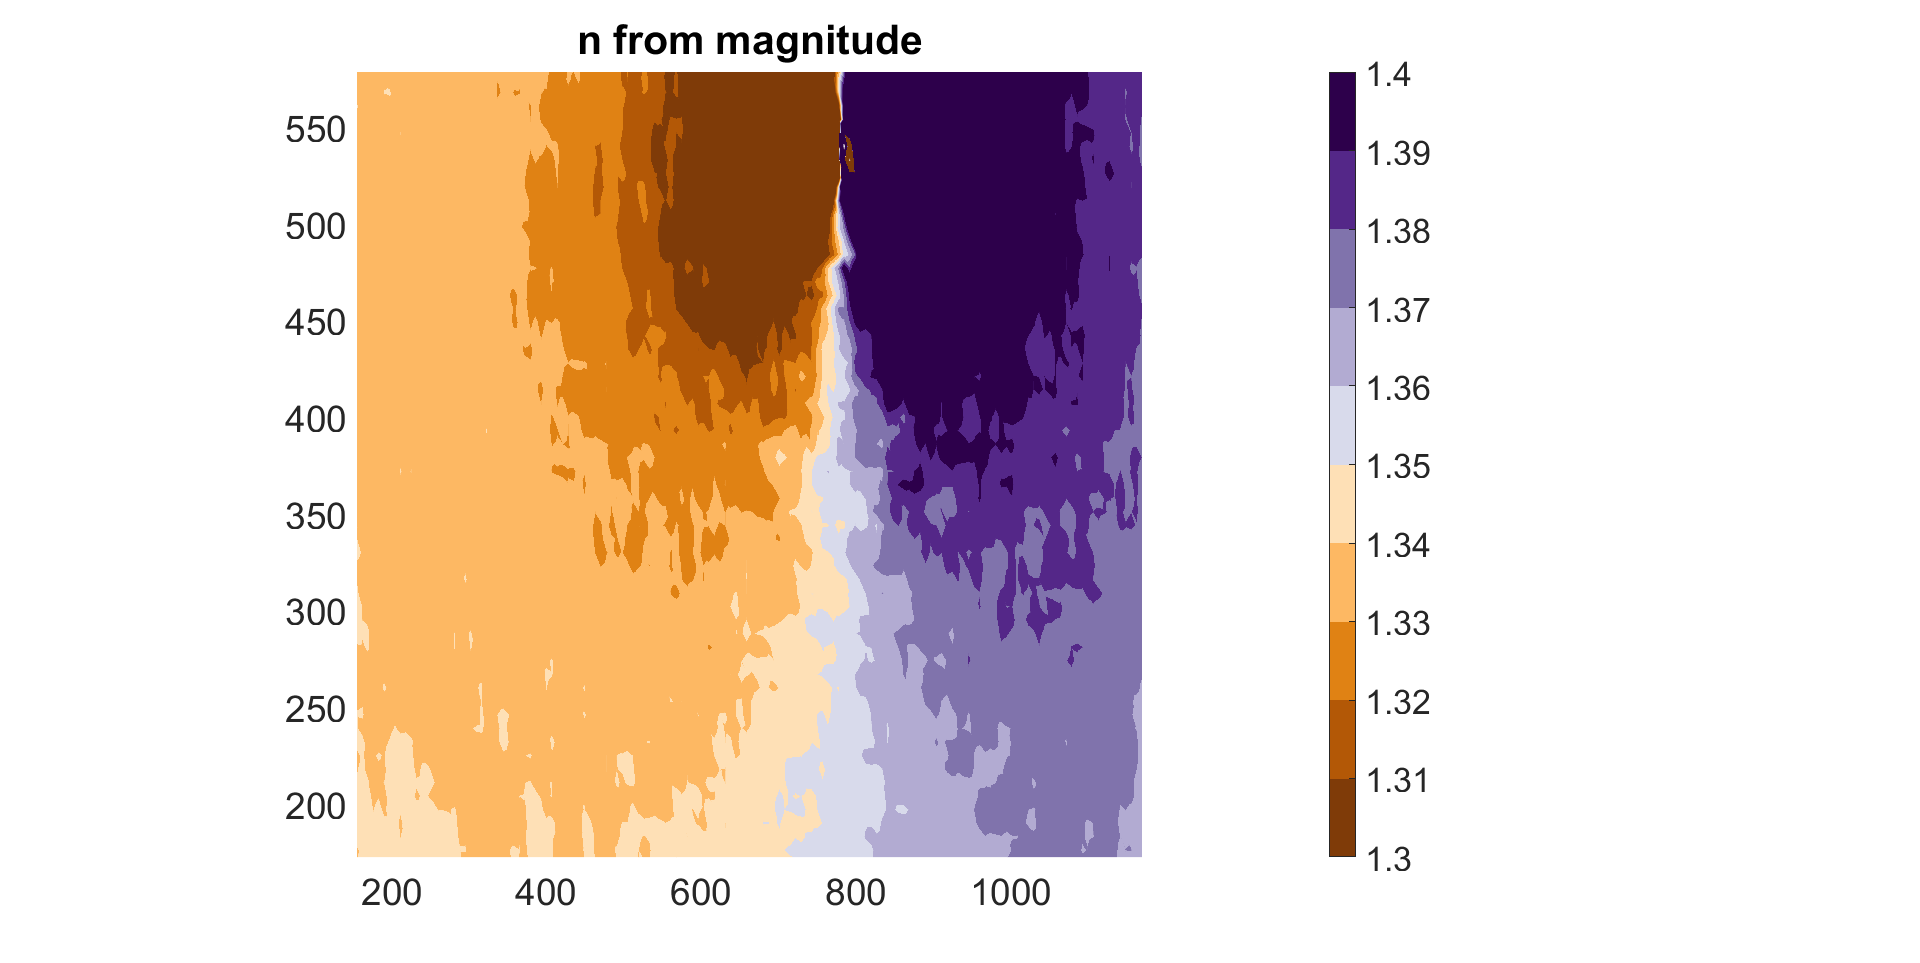
\includegraphics[width=\linewidth]{nfrommagndata.png}
\caption{Example of Index of Refraction determined Data.}
\label{fig:nfrommdataexample}
\end{figure}


\clearpage
\section{Experimental Set-up}

\subsection{Equipment}

\subsection{Error Sources}

\begin{table}[htbp]
\caption{Estimated Error Magnitudes for a \SI{100}{\milli\metre} field of view. Copied from MatchID.}
\label{tab:esterrmagn}
\begin{tabular}{@{}llr@{}} \toprule
2D Error	& Estimated Error (pixels)	& Notes \\ \midrule 
Contrast/Noise & 0.01 & Easiest to determine and minimize. \\
Interpolant Bias & 0.01 to 0.001 & Depends on noise and interpolant. \\
Lighting Variation & 0.005 & If using ZNNSD. \\
Subset size / Shape & linear fit to  &  Depends on underlying \\
 \hspace{.3cm} function & displacement field & displacement field.  \\
Optical distortions & 1+ & Depends on lens and distance moved.\\
 \hspace{.3cm} without corrections	&	& \\
Image Blur	& 0.001 & If blur is constant for all frames.\\
Turbulence/Shockwaves & $\sim$ 0.01 to 2+ & Depends on lightning and lab environment. \\
Out-of-Plane	& $\sim$ 0.5	& Depends on magnification and motion. \\
Lack of Perpendicularity	& $\sim$ 0.5	& Depends on tilt and motion. \\
System Resolution	& Small	& Increases subset size.\\
Aliasing	& $\sim$ 0.005	& Adds noise to the image.\\ \bottomrule
\end{tabular}
\end{table}

\subsection{Corrections}

\section{Experimental Results}

\subsection{Constant Density, Single Layer Fluids}

\subsection{Constant Density, Multiple Layers Fluids}

\subsection{Stratified Fluids}

\end{document}